\chapter{Programmentwurf}

In diesem Kapitel m"ochte der Autor die Entwicklung des Gesamtprogramms er"ortern.
Es wird ein "Uberblick "uber das umfassende Konzept des internen Aufbaus gegeben um anschlie\ss end auf die konkrete Umsetzung der einzelnen Bestandteile einzugehen.
Demzufolge sind die kommenden Abschnitte nach den Programmkomponenten gegliedert.
In jedem einzelnen Abschnitt wird auf drei Punkte eingegangen:
\begin{itemize}
	\item Grundlegende Idee und Designkonzept
	\item Implementierungsdetails
	\item Tests zur Validierung der einzelnen Komponente
\end{itemize}
Es sei darauf hingewiesen, dass die eigentlichen Entwicklung und Implementierung nicht Komponentenweise, sondern nach entsprechenden Funktionalit"aten statt findet.
Das Einbinden einer bestimmten Funktionalit"at betrifft oft mehrere Komponenten und ihr Zusammenspiel, wodurch der Ausbau der einzelnen Bestandteile parallel geschieht.
Die Gliederung dieses Kapitels nach den Programmteilen dient jedeglich der "Ubersichtlichkeit.

\section{"Uberblick "uber das Gesamtprogramm}

-- theoretische beschreibung des gesamtkonzeptes
-- auflisten der subkomponenten
-- graphische "Ubersicht der Bestandteile

\section{Datenbehandlung}

Es existieren \cite{Schlogl2009}

vorhandene Datensatzformate
	-- kurze "ubersicht
	-- insbesondere vergleich unisens - wfdb - edf

wahl von unisens begruenden
	-- menschlich editierbar (xml header)
	-- verzeichnis vs eine datei ist vernachl"assigbar
	-- reine sensordaten importierbar
	-- implementierung vorhanden
	-- f"ur matlab und java

\subsection{Unisens}

Das vom Forschungszentrum Informatik und Institut f"ur Technik der Informationsverarbeitung der Universit"at Karlsruhe entwickelte Datenformat Unisens dient der Speicherung und der Dokumentation von Sensordaten.
Unisens ist konzipiert, Daten verschiedener Sensoren innerhalb eines Datensatzes zu speichern.
Ein Datensatz ist im Dateisystem durch ein eigenes Verzeichnis und eine Headerdatei \verb|unisens.xml| hinterlegt.
In der Headerdatei werden alle Informationen "uber die Bestandteile des Datensatzes, deren Formatierung und ihre semantischen Zusammenh"ange gespeichert.
Messwerte eines Sensors werden "ublicherweise in einer Datendatei innerhalb des Datensatzverzeichnisses abgespeichert.
Eine solche Datendatei wird als \emph{Entry} in dem Datensatz bezeichnet.
Alle Metainformationen zu den Sensordaten werden in der Headerdatei abgspeichert, so dass die Datendateien selbst immer nur die reinen Messdaten enthalten.
Als m"ogliche Sensordaten werden sowohl kontinuierlich abgetastete Signale als auch ereignisorientierte Daten unterst"utzt.
Unisens unterscheidet zwischen vier Arten von Daten:
\begin{description}
	\item[Signale \emph{(Signal)}] \hfill \\
		Signale sind "aquidistant abgetastete, numerische Messdaten.
		Sie zeichnen sich durch eine beliebige aber konstante Abtastrate und Abtastaufl"osung aus.
		Zudem k"onnen Signale aus mehreren Kan"alen bestehen, die alle in ein und derselben Datei abgespeichert werden.
		Alle Kan"ale desselben Signals haben auch dieselbe Abtastrate und -aufl"osung.
	\item[Ereignisse \emph{(Event)}] \hfill \\
		Ereignisse sind diskrete Zeitpunkte die mit einer textlichen Beschreibung versehen sind. (z.B. Triggersignale)
		Sie zeichnen sich durch einen Zeitstempel und einer kurzen Beschreibung aus.
		Optional k"onnen noch Kommentare zu einem Ereignis hinzugef"ugt werden.
	\item[Einzelwerte \emph{(Value)}] \hfill \\
		Einzelwerte sind eine Kombination der beiden oben genannten Datenarten.
		Sie beinhalten numerische Werte die zu bestimmten Zeitpunkten aufgenommen wurden.
		Mit Einzelwerten ist es m"oglich Daten zu speichern, die nicht in festen Zeitintervallen gemessen werden.
	\item[Propriet"are Daten \emph{(Custom data)}] \hfill \\
		Mit dieser Art k"onnen anwendungsspezifisch Daten gespeichert werden, die durch die drei oben genannten Arten nicht erfasst werden k"onnen.
		So k"onnen beispielsweise schematische Darstellungen des Messaufbaus als Bilddateien oder Patienteakten in Form von Textdateien dem Datensatz hinzugef"ugt werden.
\end{description}
Eine detailiertere Beschreibung des Formates kann der offiziellen Dokumentation \cite{Ottenbacher2010} entnommen werden.

\subsubsection{Details der Implementierung}

In diesem Abschnitt wird kurz auf einige Details der Umsetzung des Unisens-Formates eingegangen.
Das Unisens-Paket ist in Java implementiert und wird unter der \emph{\ac{LGPL}} zur Verf"ugung gestellt.
Die bereit gestellte Bibliothek ist auf zwei Einzeldateien aufgeteilt: \verb|org.unisens.jar| und \verb|org.unisens.ri.jar|.
Bei der ersten Datei handelt es sich um die Definiton des Unisensformates und seiner Bestandteile als Javalassenstruktur.
Diese Definition erfolgt haupts"achlich als \emph{Interface}klassen und legt die Schnittstellen zwischen den einzelnen Bestandteilen fest.
Eine "Ubersicht der Klassenstruktur und der von au\ss en ersichtlichen Attribute ist in Abbildung \ref{pic:unisens_interface} auf Seite \pageref{pic:unisens_interface} dargestellt.
\begin{sidewaysfigure}
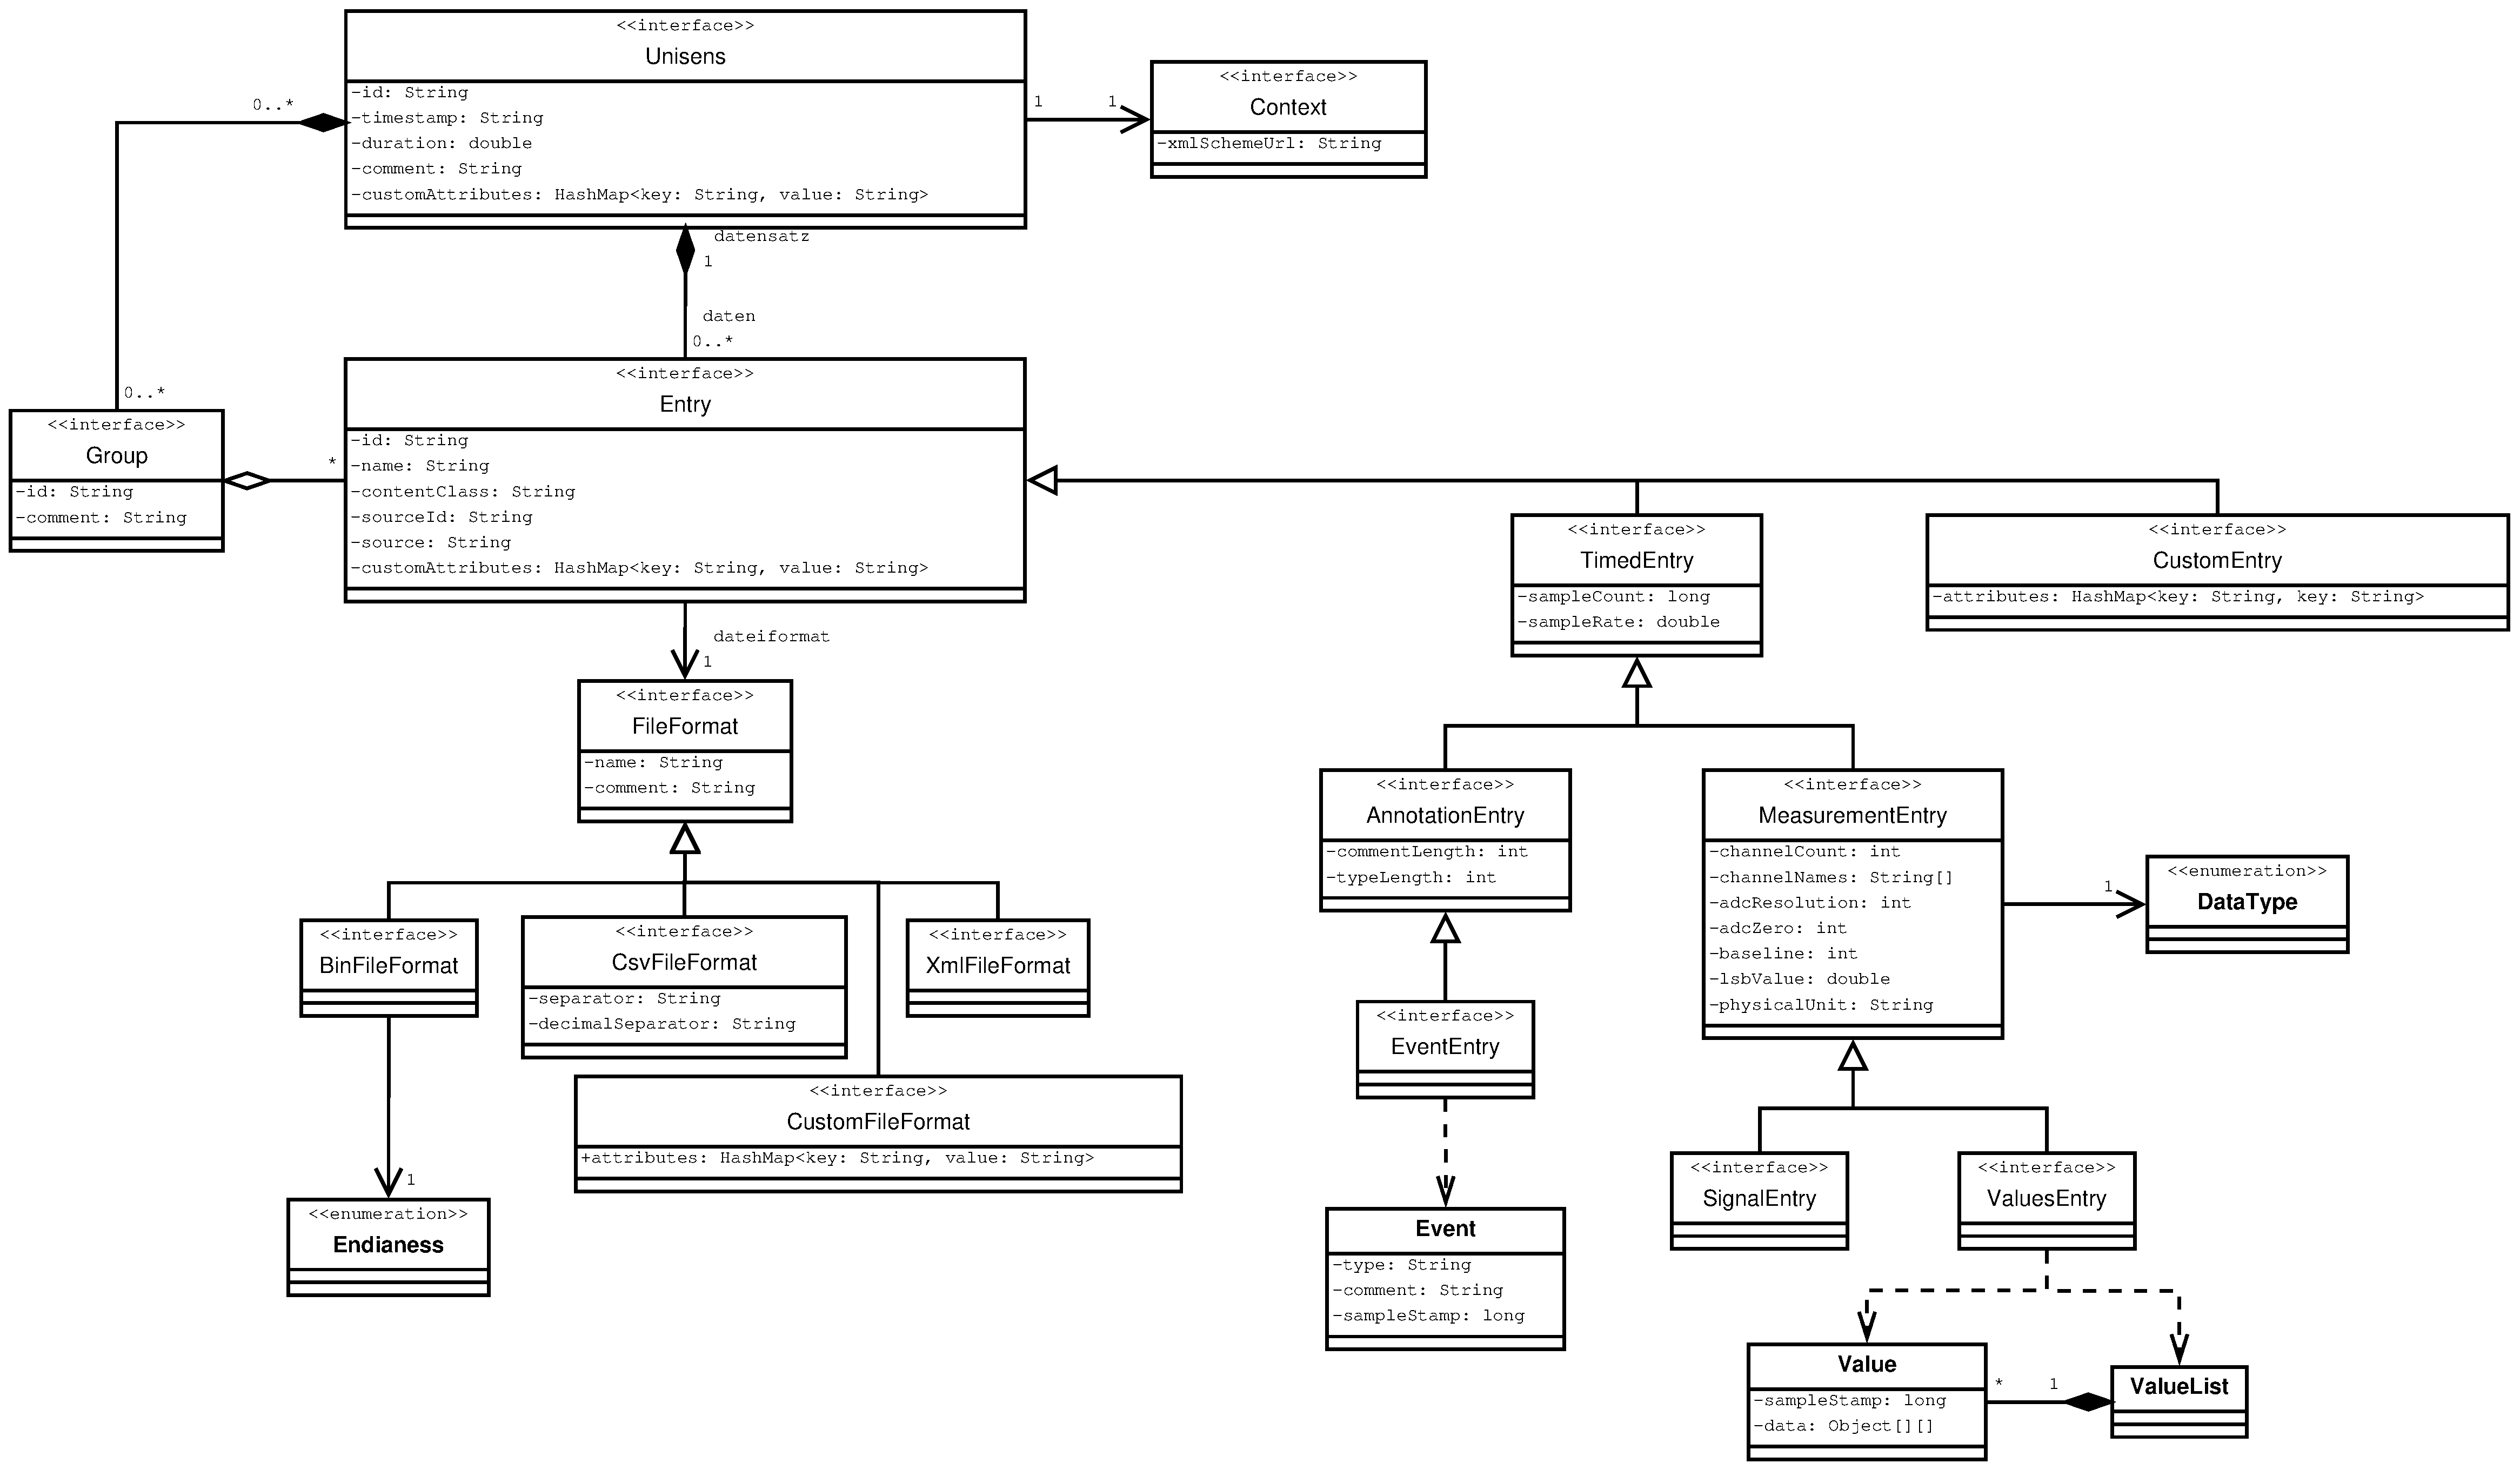
\includegraphics[width=\textwidth]{bilder/unisens_interface_.eps}
\caption{Klassen"ubersicht der von Unisens definierten Schnittstellen}
\label{pic:unisens_interface}
\end{sidewaysfigure}
Die vom Unisensformat unterst"utzten Signalarten sind auch in der Klassenstruktur erkennbar:
\begin{table}[h]
\centering
\begin{tabular}{|c|c|}
	\hline Signale & \verb|SignalEntry| \\
	\hline Ereignisse & \verb|EventEntry| \\
	\hline Einzelwerte & \verb|ValuesEntry| \\
	\hline Propriet"are Daten & \verb|CustomEntry| \\
	\hline
\end{tabular}
\caption{Signalarten und ihre repr"asentierenden Klassen}
\label{tab:signal_klassen}
\end{table}

Aufgrund der Ableitung der Klassen \verb|EventEntry| und \verb|ValuesEntry| von \verb|TimedEntry| ist ersichtlich, dass die Zeitpunkte von Ereignisdaten und Einzelwertdaten "uber eine virtuelle Abtastrate bestimmt werden.
Der Zeitpunkt eines jeden \emph{Event}- oder \emph{Value}-Eintrags ist als ganzzahlige Samplenummer dieser Abtastrate gespeichert.
Die Zeit eines Ereignisses, relativ zum Messbeginn, errechnet sich somit $Zeitpunkt = {Samplenummer \over Abtastrate}$.
M"ochte man die M"oglichkeit Ereignisse f"ur jeden beliebigen Datenpunkt eines Datensatzes zuordnen zu k"onnen, dann muss die virtuelle Abtastrate als das kleinste gemeinsame Vielfache aller vorhandenen Abtastraten gew"ahlt werden.

Die Schnittstellendefinition des Unisensformats stellt nur Methoden zum Lesen und Anh"angen von Datenpunkten an den Datensatz bereit.
Somit wird ein Einf"ugen, L"oschen oder Ver"andern von Datenpunkten innerhalb eines Dateneintrags nicht unterst"utzt.
Sollen diese Funktionen vorhanden sein, so muss diese Funktionalit"at selbst implementiert werden.

Die eigentliche Umsetzung der Funktionalit"at ist in der zweiten Datei abgespeichert.
Im Folgenden soll sich der Begriff Referenzimplementierung auf diese funktionelle Umsetzung beziehen.
Die Klassen der Referenzimplementierung bestehen aus den Klassennamen der Schnittstellendefinition und dem Suffix "`Impl"' (z.B. Objekte die den Datensatz darstellen haben die Klasse \verb|UnisensImpl|).
Wenn man schon vorhandene Unisensdatens"atze benutzen m"ochte reicht es aus, die Schnittstellendefinition zu kennen und zu nutzen.
Sollen hingegen konkret Objekte erstellt werden, muss auf die Referenzimplementierung zur"uckgegriffen werden.

Durch einen Fehler in der Referenzimplementierung kann es vorkommen, dass beim Laden eines vorhandenen Unisensdatensatzes in dem Gruppen definiert sind eine \verb|NullPointerException| auftritt.
Insbesondere tritt dieser Fehler auf, wenn innerhalb der Headerdatei der Gruppeneintrag nicht hinter den Dateneintr"agen steht.

\subsection{Interne Datenstruktur}

Kapselung von unisens in wrapperklassen -> erweiterung und vereinfachung der funktionalit"at

daten"ubergabe an visualisierung mithilfe der controller

\subsection{Dateibehandlung}

%\subsection{Speichermanagement}

%\section{Allgemeine Programmstruktur}

\section{Benutzerf"uhrung}

\subsection{Grafische Buntzeroberfl\"ache}

\subsection{Datenvisualisierung}

%% EOF %%%%%%%%%%%%%%%%%%%%%%%%%%%%%%%%%%%%%%%%%%%%%%%%%%%%%%
